\subsection{Configuration et modification du programme}

Le tableau~\ref{tab:initial_settings} présente les paramètres de notre première tentative de résolution du \emph{pendulum} par \emph{policy gradient}.

\begin{table}[H]
        \centering
        \begin{tabular}{@{}l l l@{}}
            \toprule
            \textbf{Study settings} & Name & Policy gradient \\
            & Critic update method & Dataset \\
            & Policy type & Squashed gaussian \\ \midrule
            \textbf{Study parameters} & Number of cycles & $ 500 $ \\
            & Number of trajectories $ m $ & $ 20 $ \\
            & Number of batches & $ 20 $ \\ \midrule
            \textbf{Algorithm settings} & Gradients methods & Sum, discount and normalize \\
            & Critic estimation method & Temporal Differences \\ \midrule
            \textbf{Learning parameters} & Reward discount $ \gamma $ & $ 0.99 $ \\
            & Adam: Actor's learning rate $ \alpha_{a} $ & $ 0.01 $ \\
            & Adam: Critic's learning rate $ \alpha_{c} $ & $ 0.01 $ \\
            & Duration of an episode & $ 200 $ steps \\
            \bottomrule
        \end{tabular}
    \caption{Tableaux de la configuration initiale de la \emph{policy gradient research}}\label{tab:initial_settings}
\end{table}

Puisque la \emph{squashed gaussien} force la politique à fournir une action entre  $ 0 $ et $ 1 $, nous décidons de doubler cette valeur dans le \emph{wrapper} du \emph{pendulum}. Cela permet à l'agent d'utiliser tout sont espace d'action.

Le problème du pendule inversé définit son état par le n--uplet $ (\cos(\theta), \sin(\theta), \dot{\theta}) $. Pour l'affichage de la critique et de l'acteur, nous pensons que $ \cos(\theta) $ et $ \dot{\theta} $ sont les paramètres les plus importants. En effet, $ \cos(\theta) $ et $ \sin(\theta) $ ont des informations similaires sur l'état. Comme la référence de $ \theta $ est en haut, le cosinus nous donne l'information sur la hauteur du pendule et le sinus nous dit de quel côté il se trouve. Puisque la récompense est calculée selon l'équation~\eqref{eq:reward}, nous savons que seul la hauteur du pendule est récompensée. Par conséquent $ \sin(\theta) $ ne fournit pas une information utile sur la récompense donnée à l'agent. Donc nous décidons d'afficher les graphes de la critique et de l'acteur en fonction de $ \cos(\theta) $ et $ \dot{\theta} $. Pour ce faire, nous ajoutons un \emph{wrapper} pour échanger la seconde composante de l'état avec la dernière.

\begin{equation}
    r(\theta, \dot{\theta}, a)= -(\theta^{2} + 0,1 \times \dot{\theta}^{2} + 0,001 \times a^{2})
    \label{eq:reward}
\end{equation}
 
\subsection{Analyses}
    
\begin{figure}[H]
    \centering
    \begin{subfigure}{0.3\textwidth}
        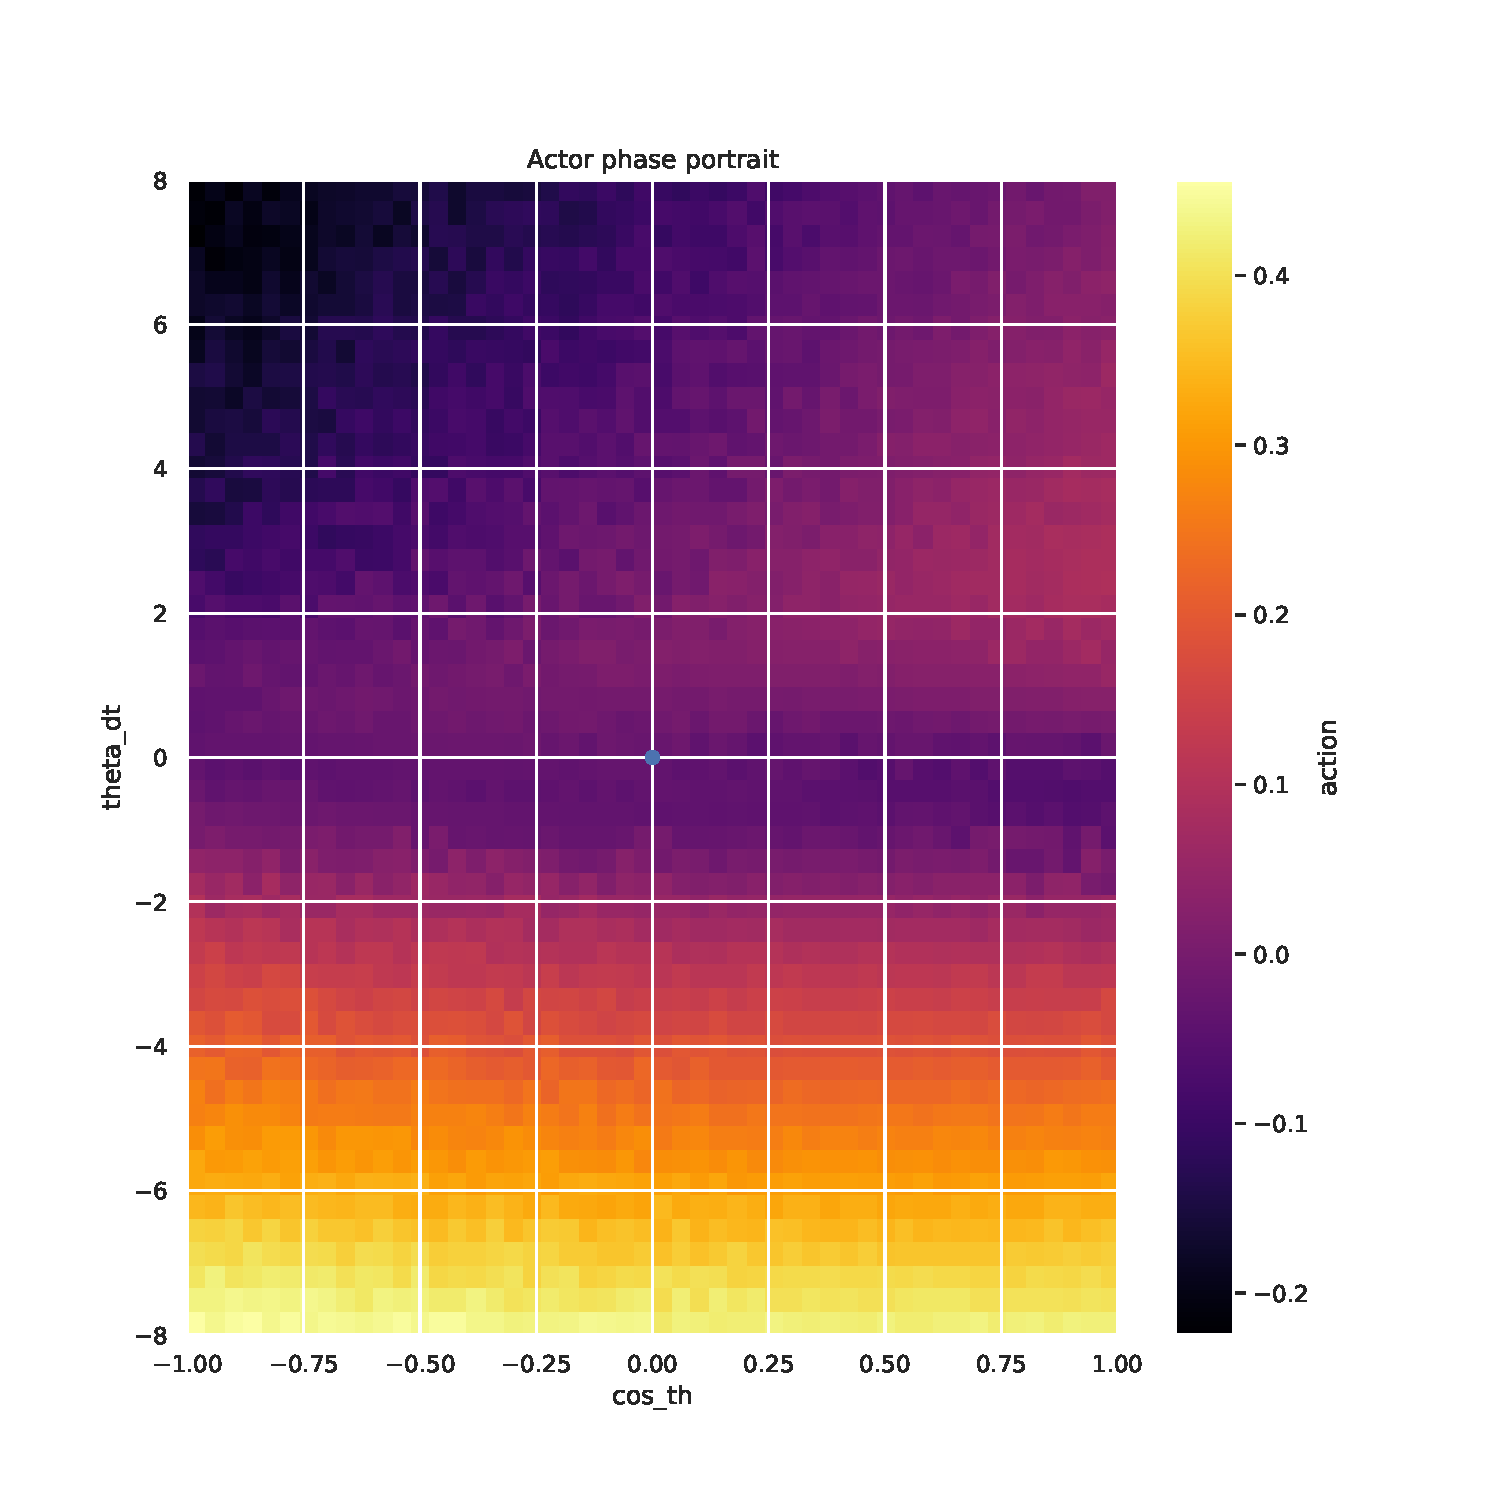
\includegraphics[width=\textwidth]{figures/prelimaire/0_actor_discount__ante_Pendulum-v0.pdf}
        \caption{Acteur naïf}
    \end{subfigure}
    \begin{subfigure}{0.3\textwidth}
        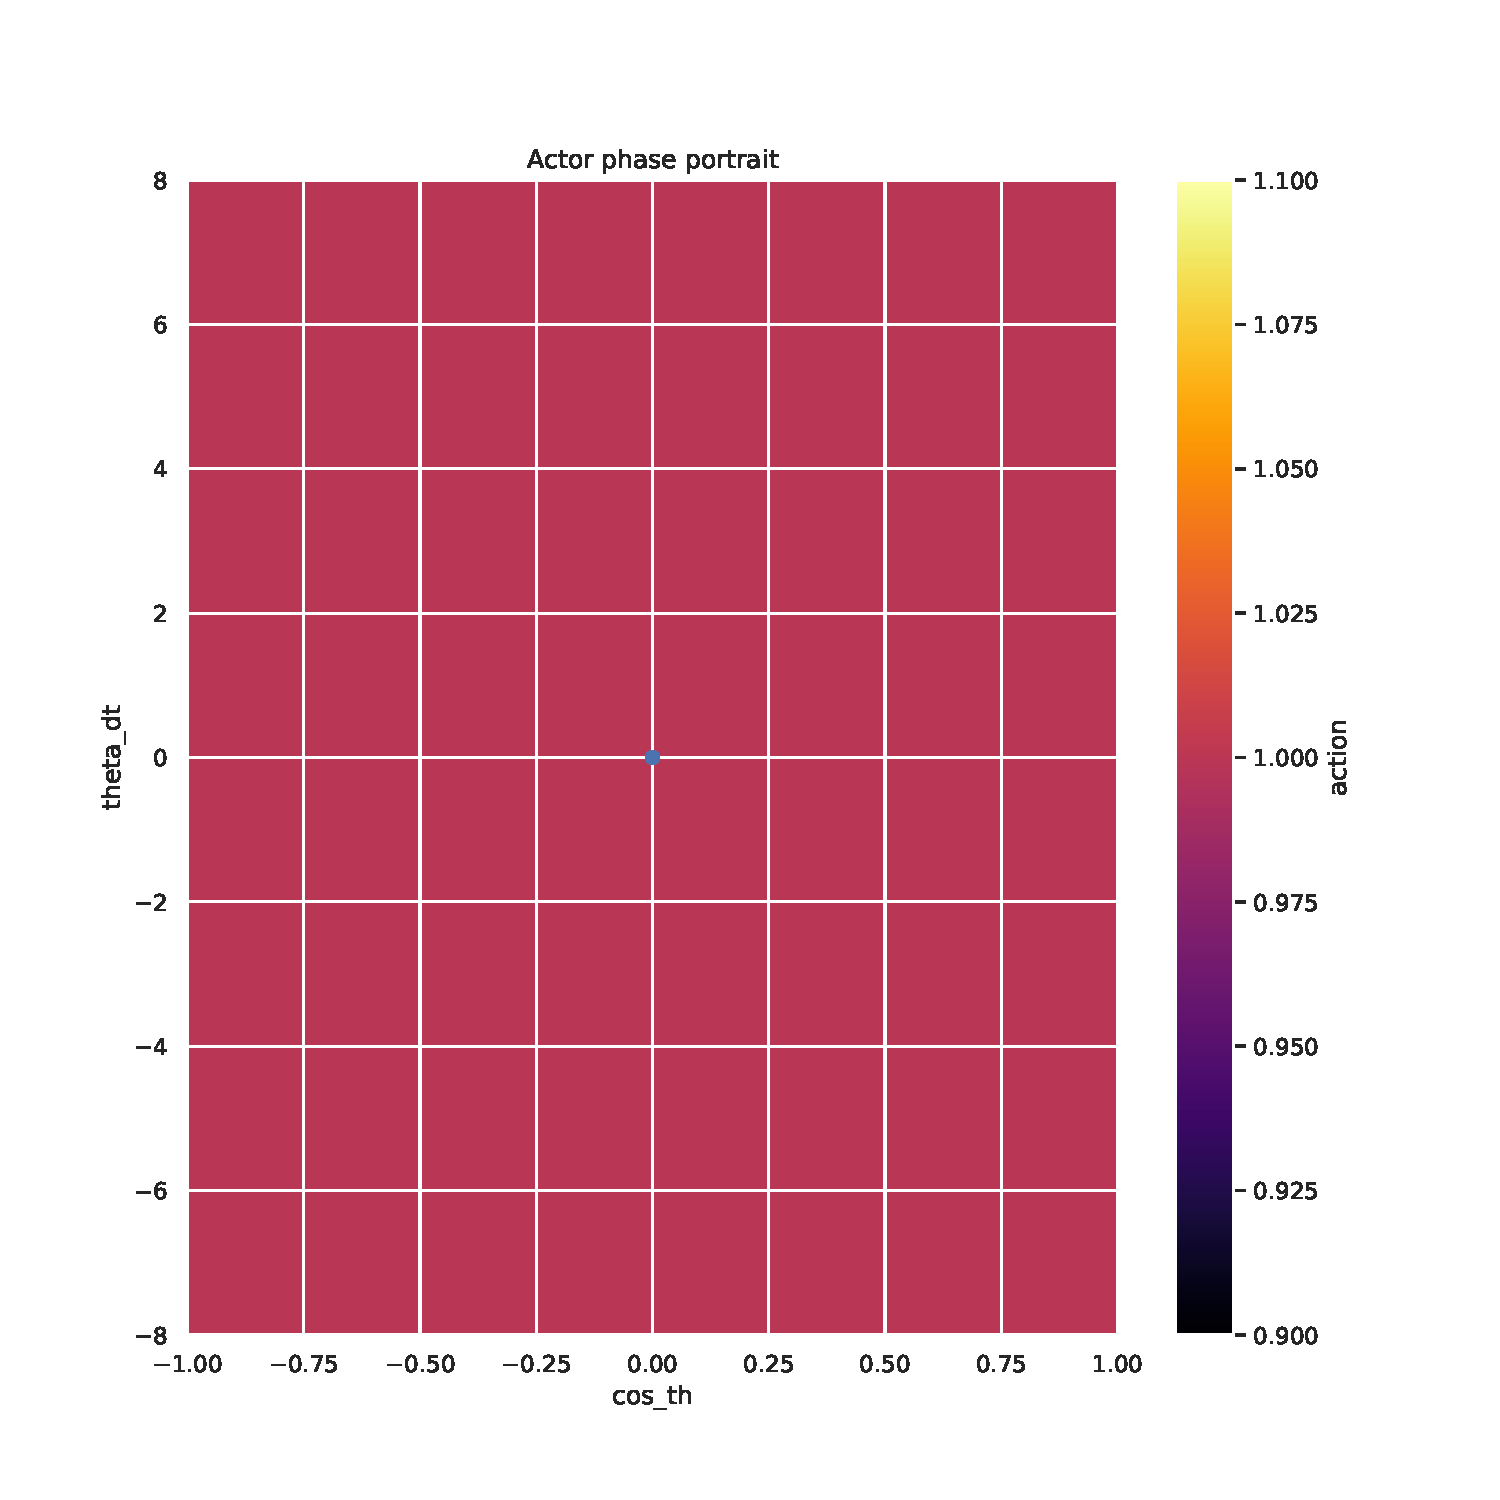
\includegraphics[width=\textwidth]{figures/prelimaire/0_actor_discount__post_Pendulum-v0.pdf}
        \caption{Acteur entraîné}
    \end{subfigure}
    \begin{subfigure}{0.3\textwidth}
        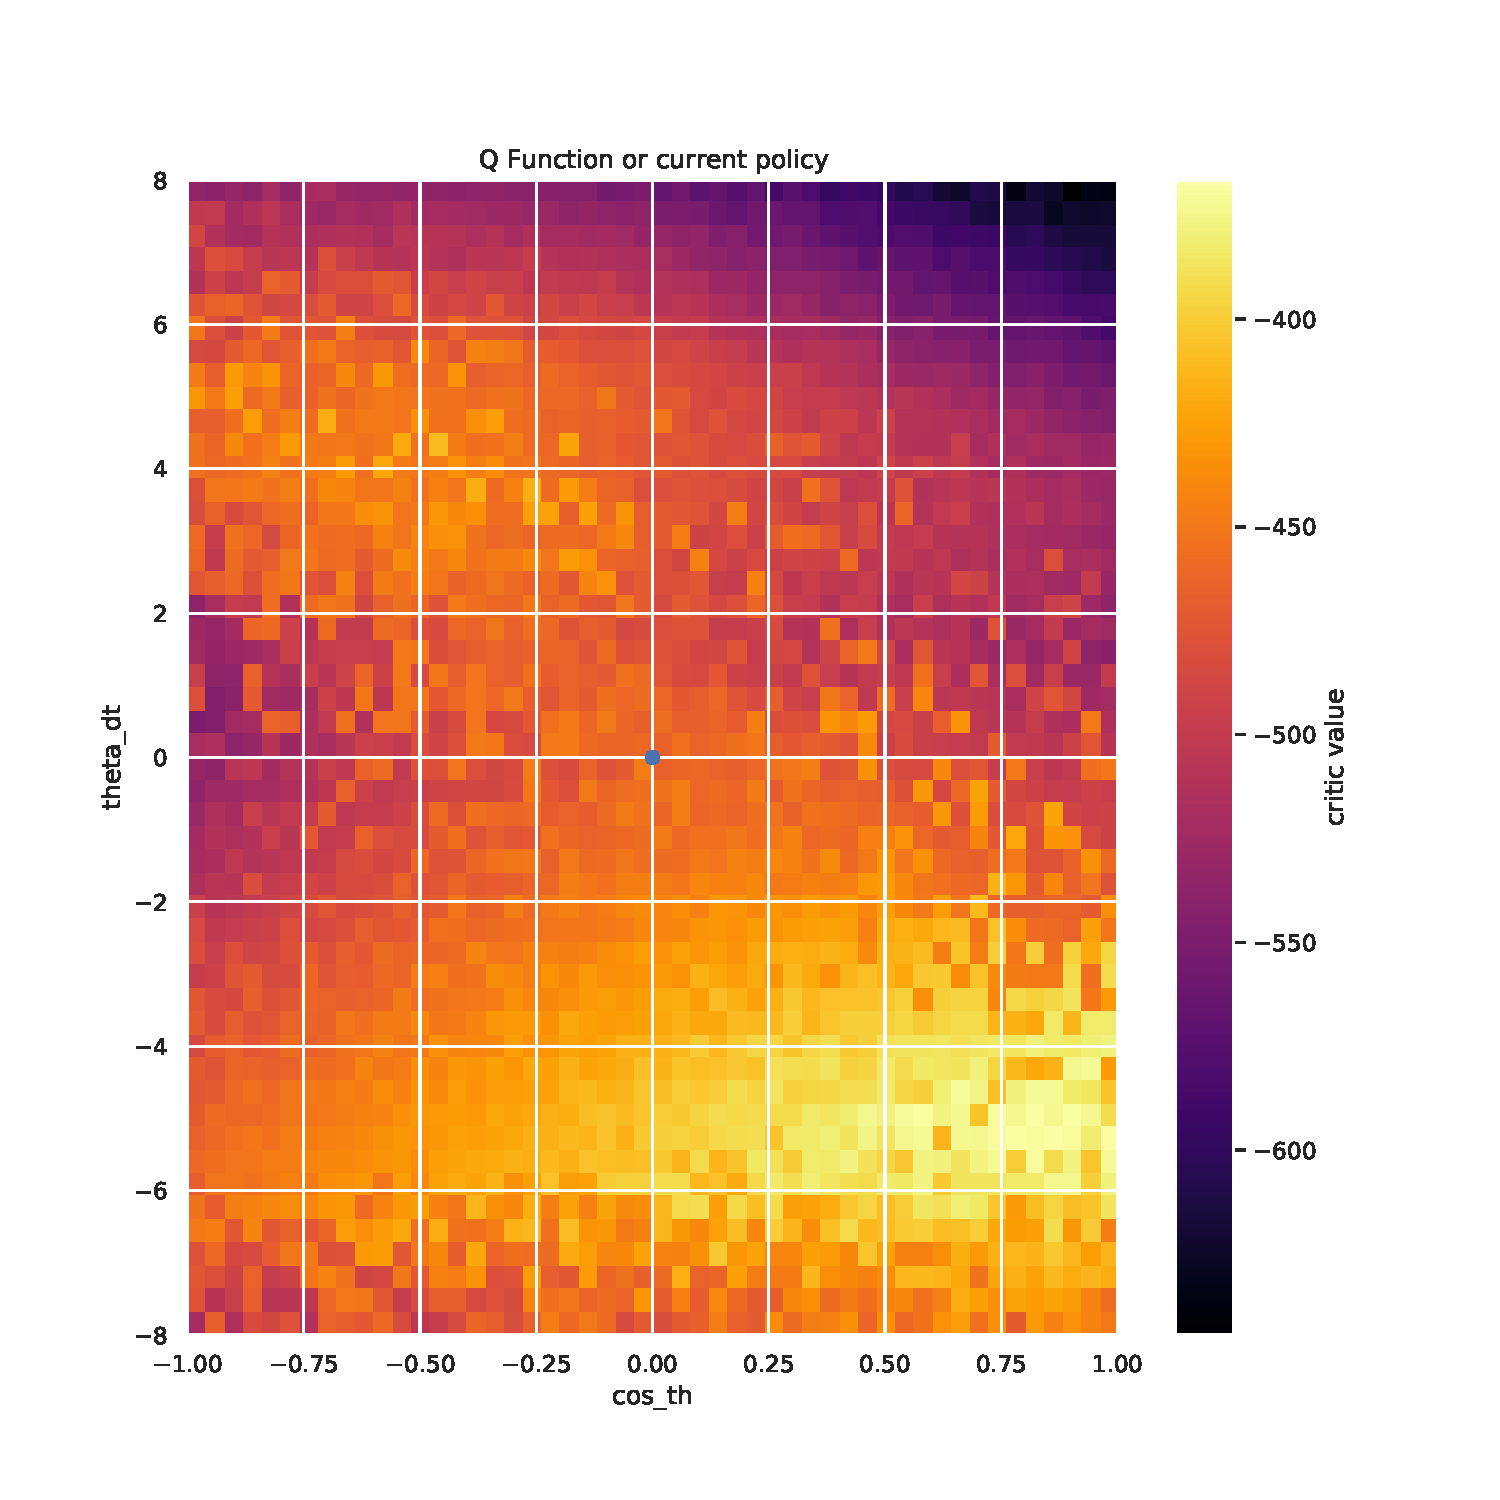
\includegraphics[width=\textwidth]{figures/prelimaire/0_critic_discount_post_Pendulum-v0.pdf}
        \caption{Critique entraînée}
    \end{subfigure}
    \caption{Valeurs de l'acteur et de la critique avec la méthode discount pour le calcul de la récompense}
    \label{fig:preli_discount}
\end{figure}

La figure~\ref{fig:preli_discount} nous montre un résultat aberrant où l'acteur converge vers une action uniforme de 1 sur l'ensemble des états qu'il peut atteindre. La \emph{heatmap} de la critique montre une préférence quand $\cos(\theta) = 1$ et c'est ce que nous voulons pour que le pendule reste à l'équilibre tout en haut. Mais on observe aussi que la zone de préférence n'est pas pour $\dot{\theta} = 0$ alors que nous souhaitons que le pendule soit immobile à la position désirée.

\begin{figure}[H]
    \centering
    \begin{subfigure}{0.3\textwidth}
        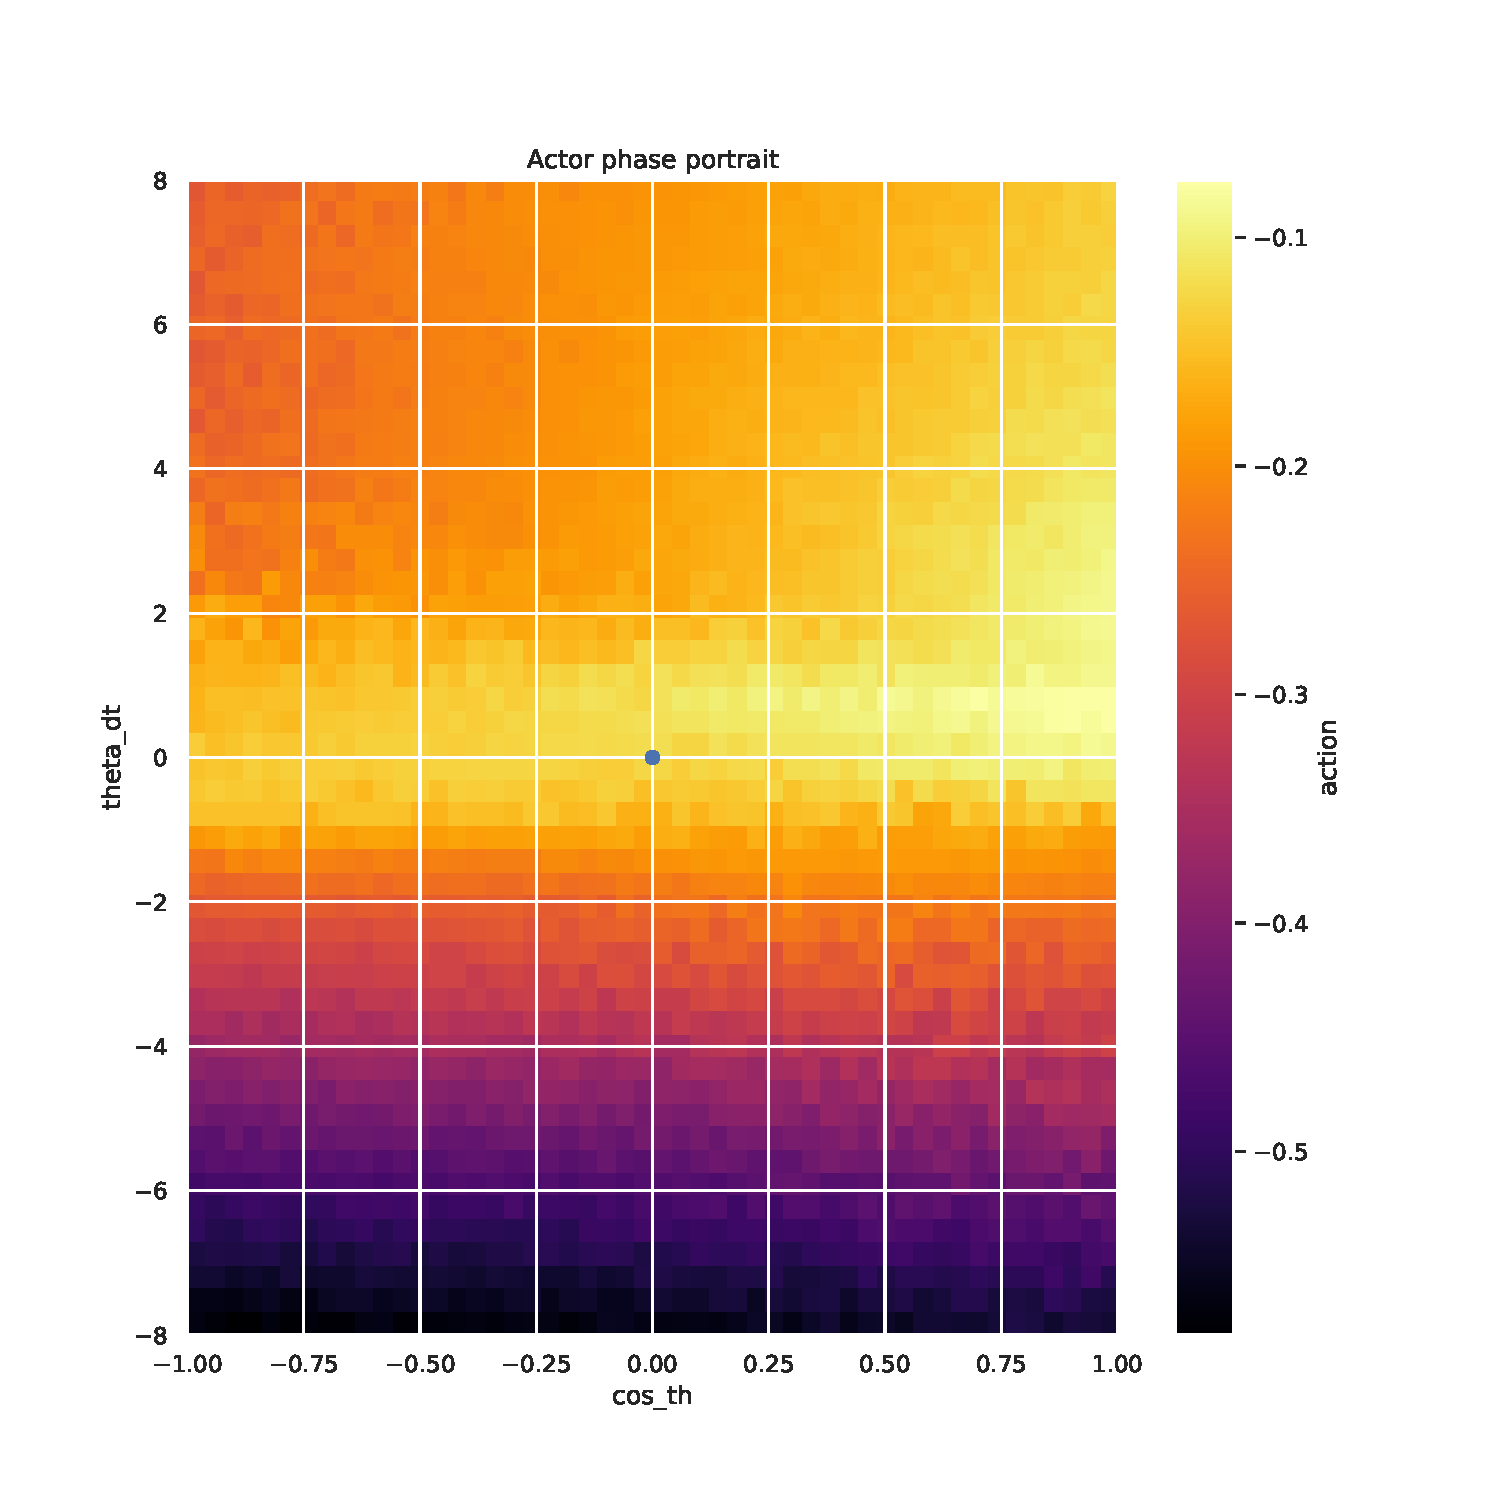
\includegraphics[width=\textwidth]{figures/prelimaire/0_actor_normalize__ante_Pendulum-v0.pdf}
        \caption{Acteur naïf}
    \end{subfigure}
    \begin{subfigure}{0.3\textwidth}
        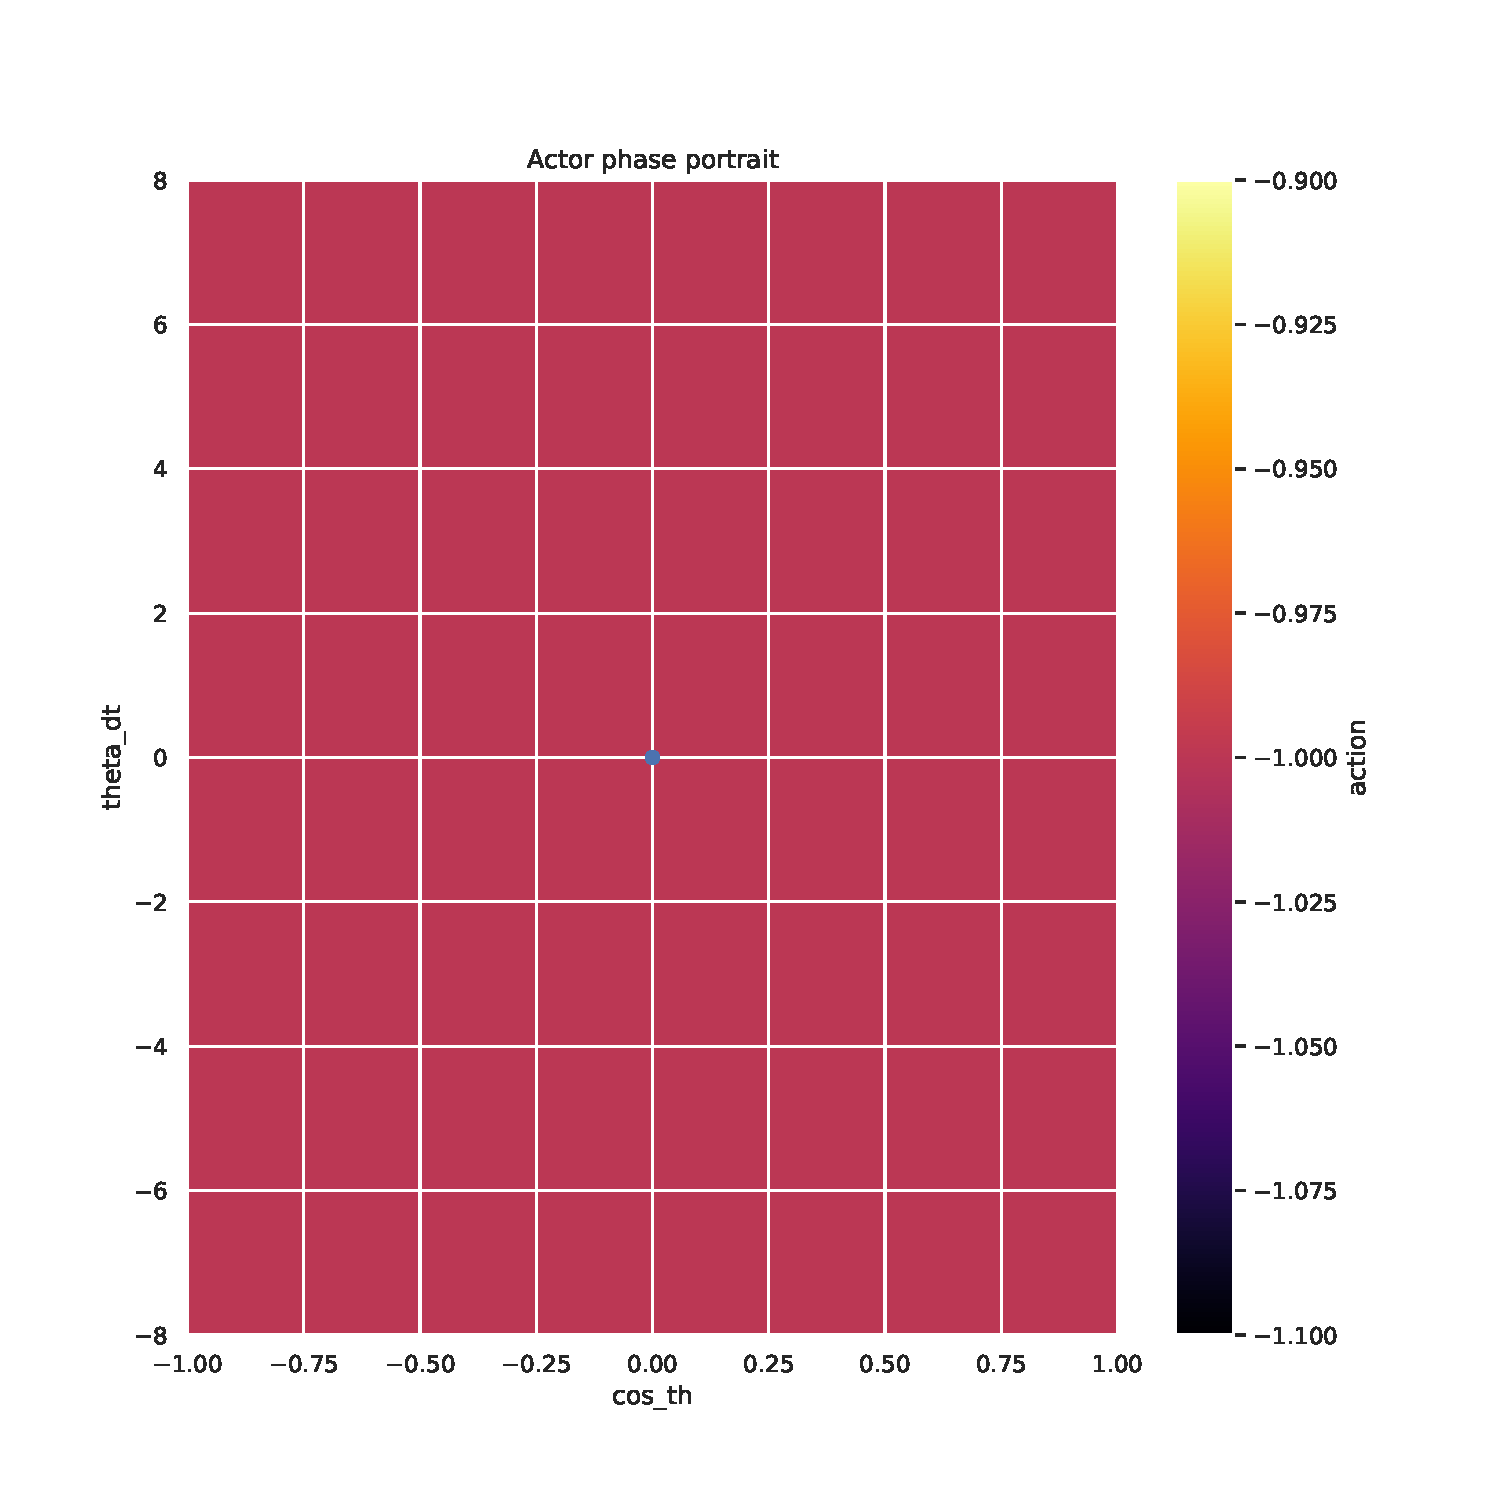
\includegraphics[width=\textwidth]{figures/prelimaire/0_actor_normalize__post_Pendulum-v0.pdf}
        \caption{Acteur entraîné}
    \end{subfigure}
    \begin{subfigure}{0.3\textwidth}
        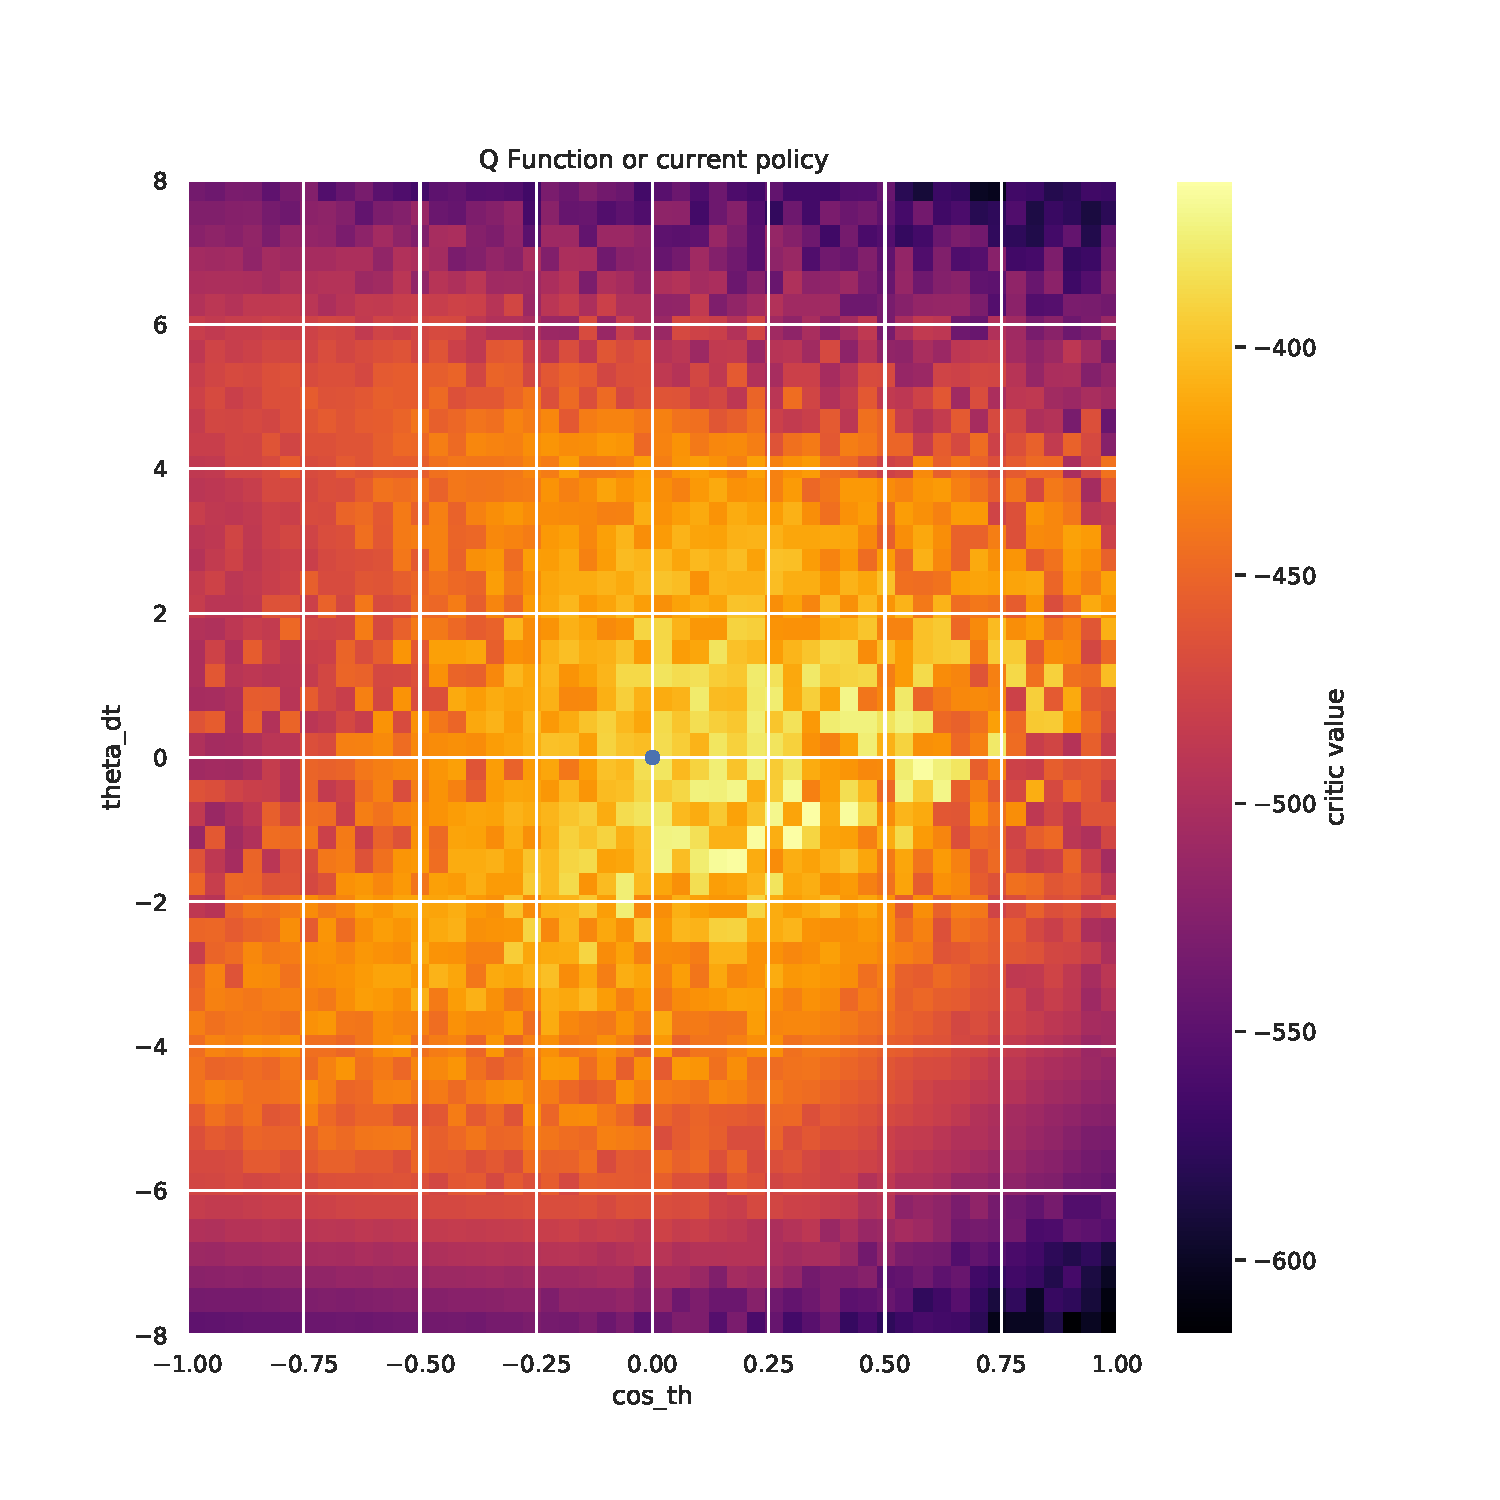
\includegraphics[width=\textwidth]{figures/prelimaire/0_critic_normalize_post_Pendulum-v0.pdf}
        \caption{Critique entraînée}
    \end{subfigure}
    \caption{Valeurs de l'acteur et de la critique avec la méthode normalise pour le calcul de la récompense}
    \label{fig:preli_normalise}
\end{figure}

La figure~\ref{fig:preli_normalise} montre le même problème pour l'acteur après entraînement où il converge vers 1 pour tous les états. Cependant, la préférence de $\dot{\theta}$ est bel et bien autour de 0 comme souhaité. Mais la valeur de préférence pour $\cos(\theta)$ n'est pas assez proche de 1 pour être caractérisée comme satisfaisante.

\begin{figure}[H]
    \centering
    \begin{subfigure}{0.3\textwidth}
        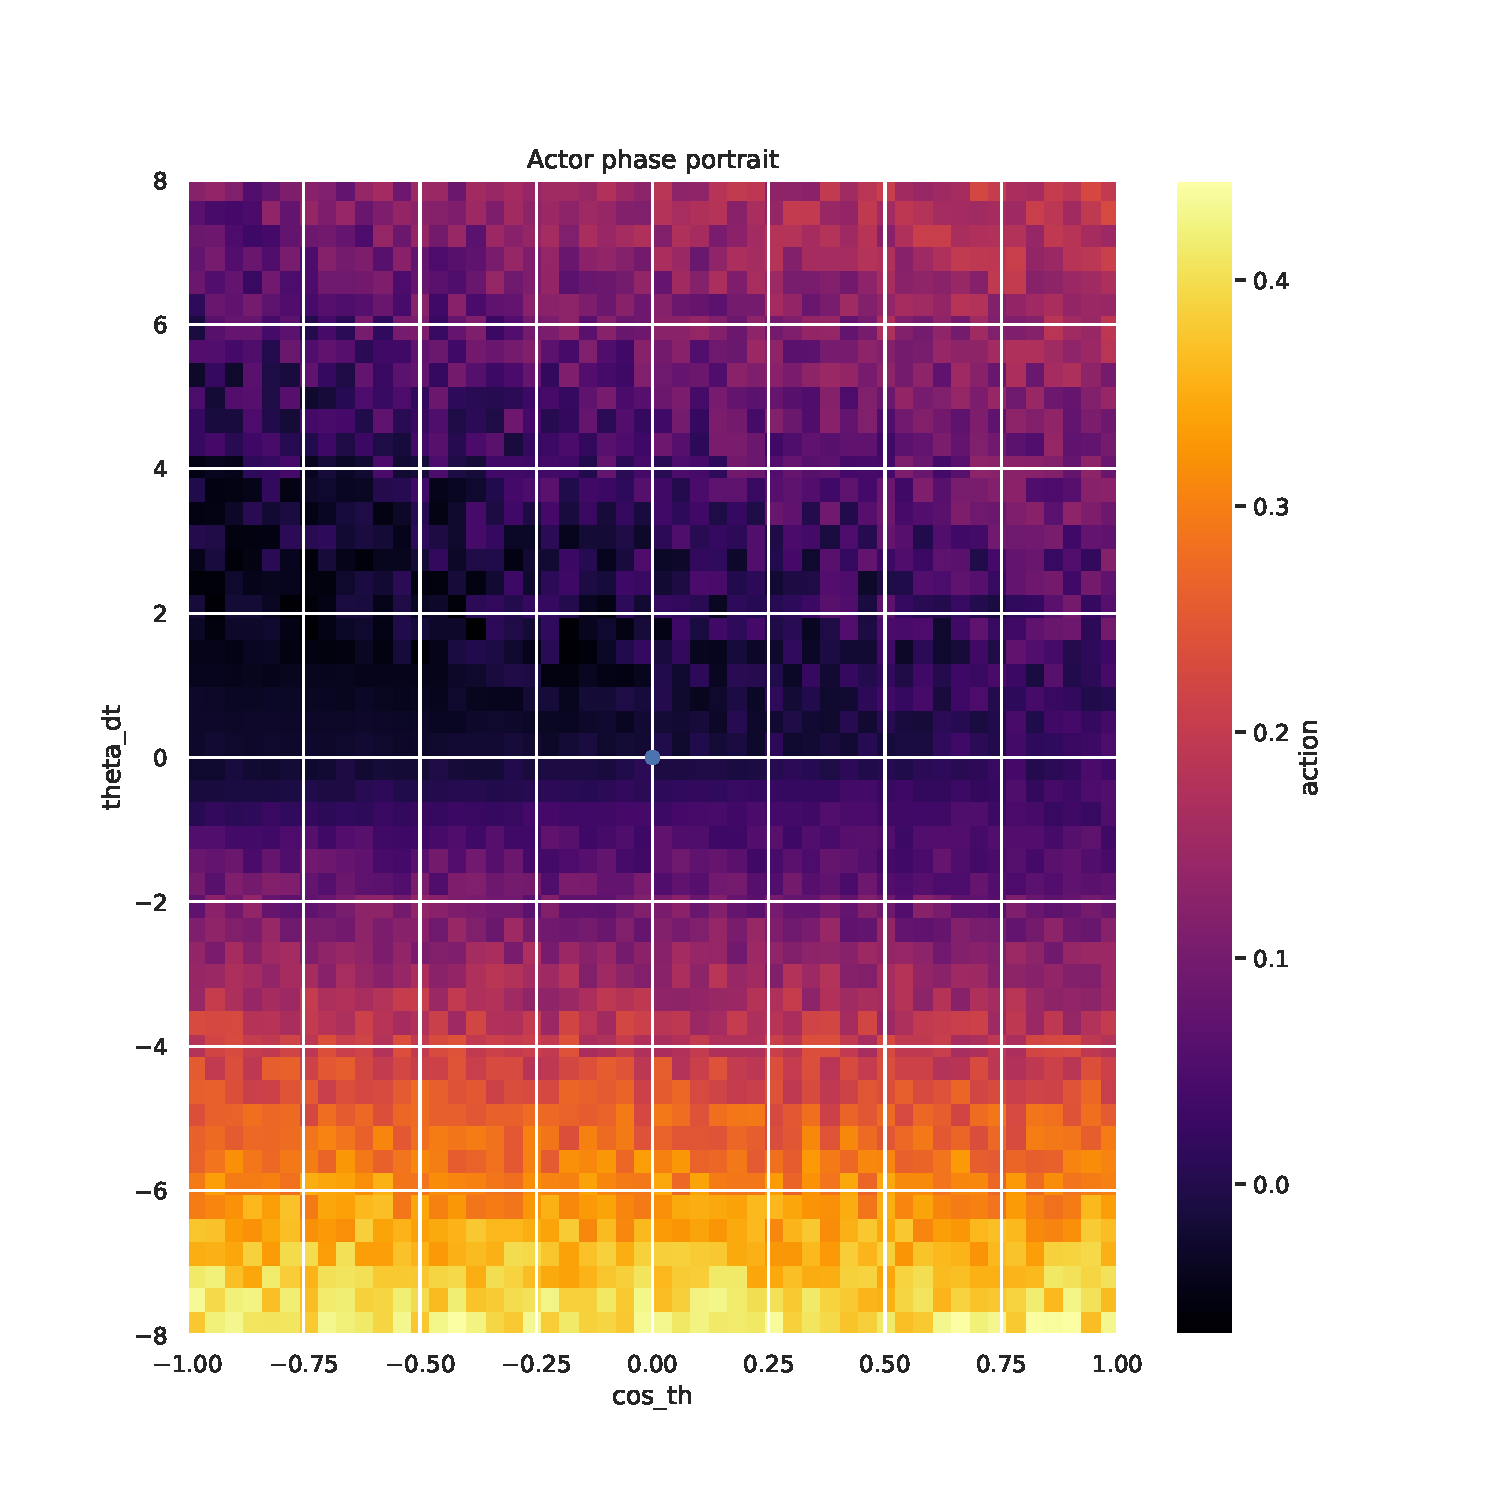
\includegraphics[width=\textwidth]{figures/prelimaire/0_actor_sum__ante_Pendulum-v0.pdf}
        \caption{Acteur naïf}
    \end{subfigure}
    \begin{subfigure}{0.3\textwidth}
        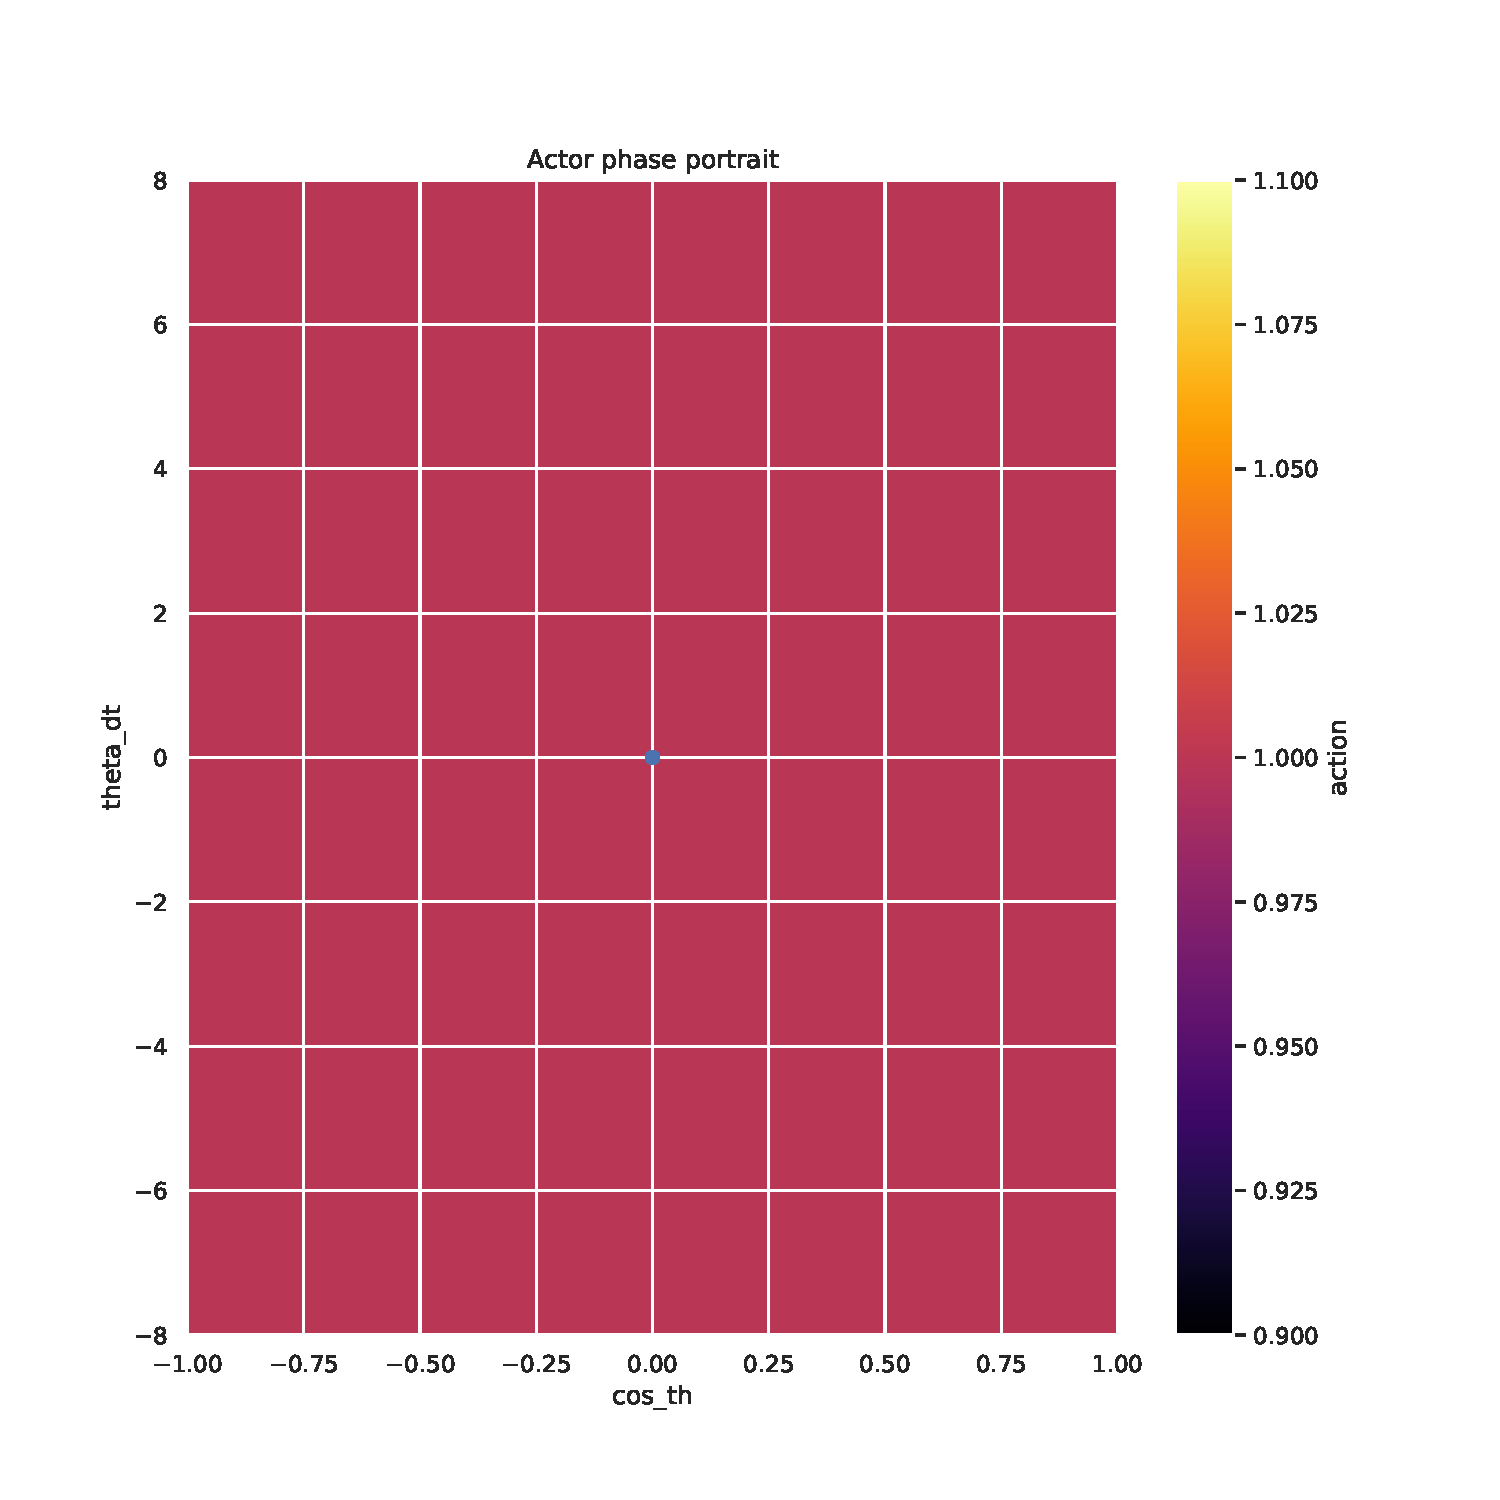
\includegraphics[width=\textwidth]{figures/prelimaire/0_actor_sum__post_Pendulum-v0.pdf}
        \caption{Acteur entraîné}
    \end{subfigure}
    \begin{subfigure}{0.3\textwidth}
        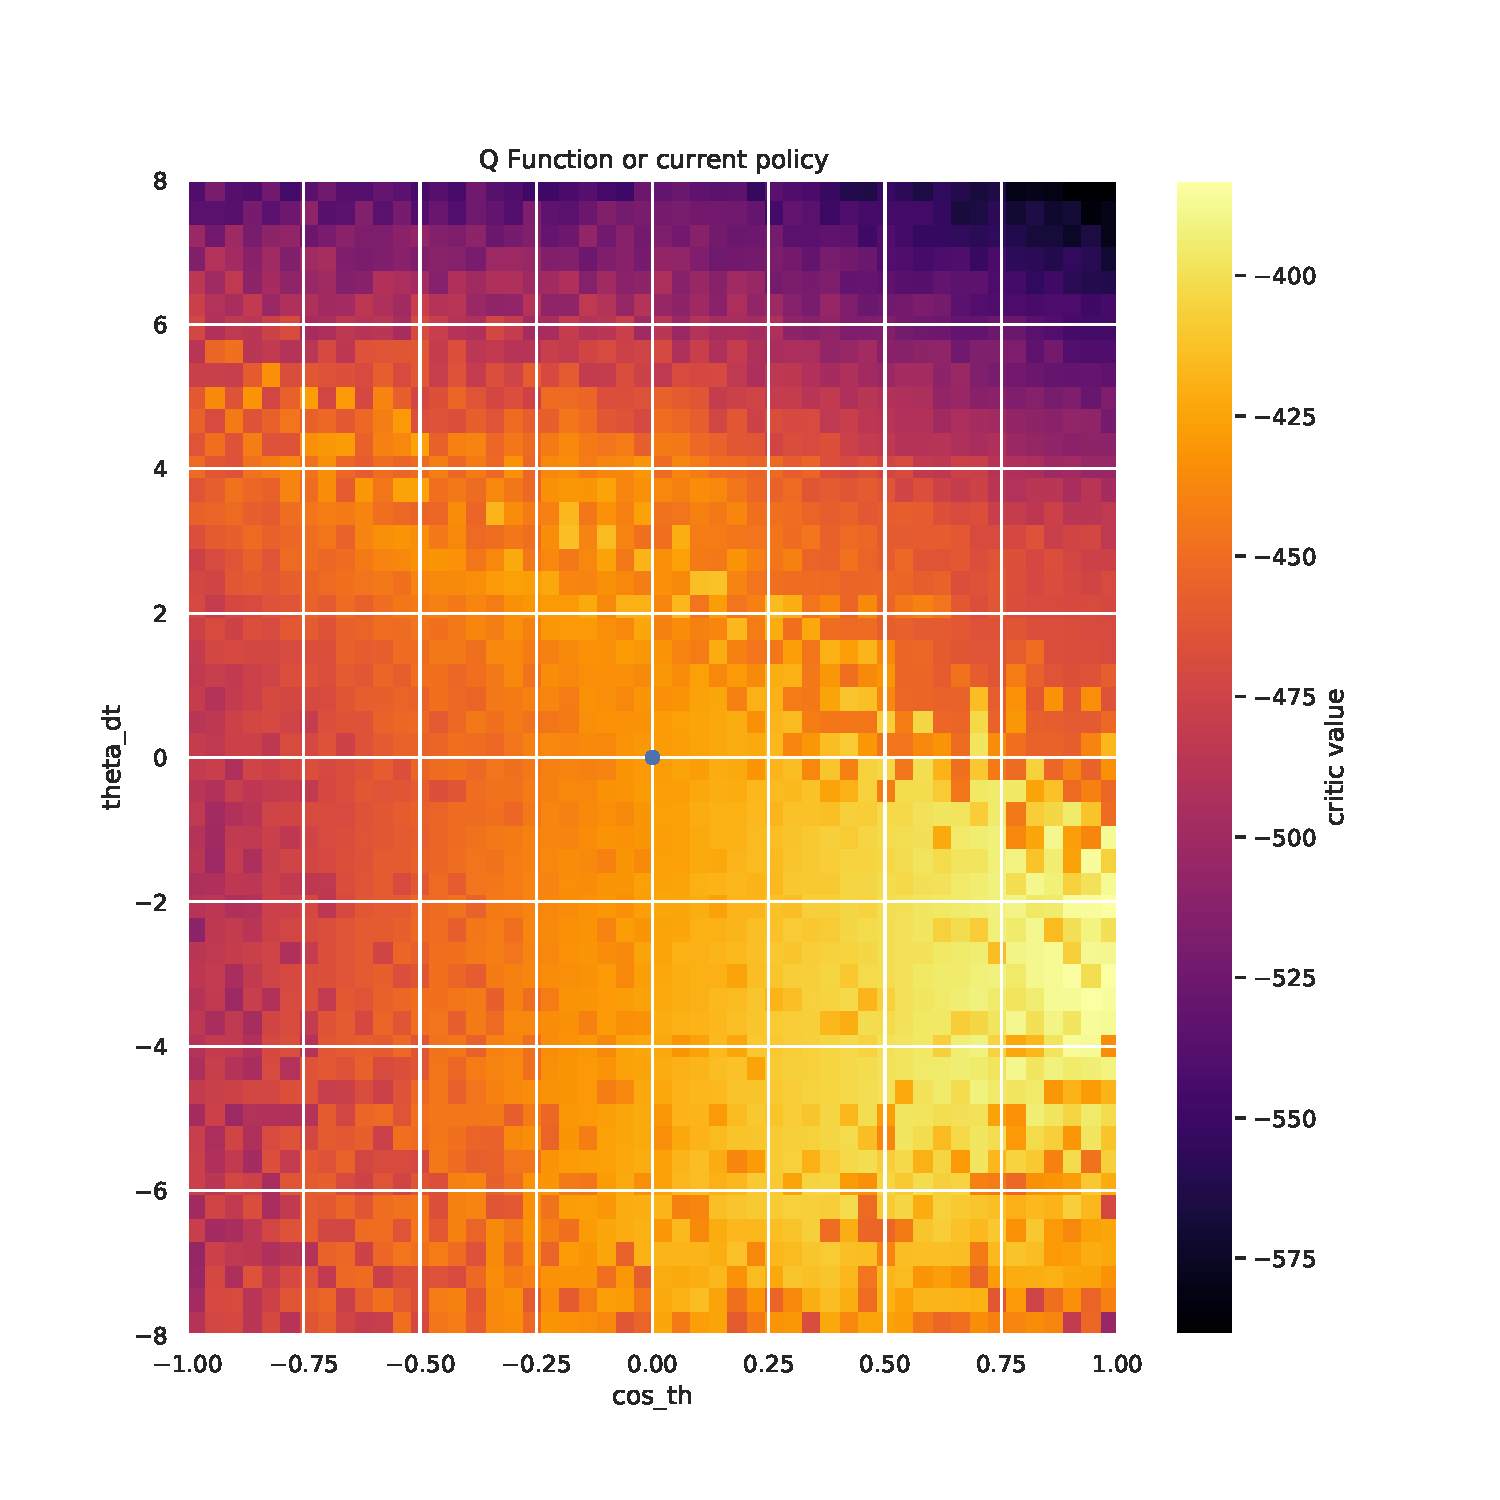
\includegraphics[width=\textwidth]{figures/prelimaire/0_critic_sum_post_Pendulum-v0.pdf}
        \caption{Critique entraînée}
    \end{subfigure}
    \caption{Valeurs de l'acteur et de la critique avec la méthode de sommation pour le calcul de la récompense}
    \label{fig:preli_sum}
\end{figure}

La figure~\ref{fig:preli_sum} présente également le résultat absurde sur l'acteur entraîné uniforme et unitaire sur l'ensemble des états. On observe par contre une zone de préférence pour $\cos(\theta) = 1$, c'est à dire la position souhaitée du pendule. Mais ici encore, pour $\dot{\theta}$, la zone de préférence n'est pas encore assez proche de 0 pour être satisfaisante.

Pour les trois méthodes de calcul de la récompense sur une trajectoire, la critique ne présente pas un maximum pour les états optimaux. Nous remarquons que les zones chaudes sont très vastes. Nous en déduisons que la critique est de mauvaise qualité par manque d'exploration.

La récompense maximum est estimée pour $\dot{\theta} \not= 0$. Donc l'agent n'a vu cette récompense que lorsque qu'il poussait à pleine vitesse. Donc le gradient de la critique a poussé la politique à toujours utiliser le couple maximum. D'où le fait que les acteurs renvoient toujours $1$ (soit le couple maximum dans le sens direct).